\chapter{Access Control}
	
	\clearpage
	Access control is the traditional center of gravity of computer security. 
	Its function is to control which principals (persons, processes, machines, . . .) 
	have access to which resources in the system — which files they can read, which 
	programs they can execute, how they share data with other principals, and so on.

	\begin{figure}[H]
		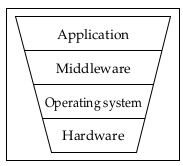
\includegraphics[scale=0.6]{pics/layers.png}
	\end{figure}

	Now one of the biggest challenges in computer security is preventing one program 
	from interfering with another. You don’t want a virus to be able to steal the 
	passwords from your browser, or to patch a banking application so as to steal 
	your money. 

	Microsoft Vista, place more emphasis on separating applications from each other; 
	even if you don’t care about security, preventing your programs from overwriting 
	each others’ configuration files should make your PC much more reliable. 

	More secure operating systems have led to ever more technical attacks on software 
	other than the operating system; you don’t want your brokerage account hacked via 
	a computer game you downloaded that later truns out to be insecure. And employers 
	would like ways of ensuring that employees’ laptops don’t pick up malware at home, 
	so it makes sense to have one partition (or virtual machine) for work and another
	for play.

	\clearpage
	\section{Operating System Access Control}

		The access controls provided with an operating system typically authenticate
		principals using a mechanism such as passwords or Kerberos, then mediate
		their access to files, communications ports and other system resources.
		Their effect can often be modelled by a {\bf matrix} of access permissions, with
		columns for files and rows for users. We’ll write {\bf r} for permission to read, 
		{\bf w} for permission to write, {\bf x} for permission to execute a program, and 
		{\bf -} for no access at all.

		\begin{figure}[H]
			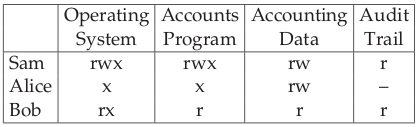
\includegraphics[scale=0.6]{pics/access1.png}
		\end{figure}

		This is often enough, but in the specific case of a bookkeeping system
		it’s not quite what we need. We want to ensure that transactions are well-
		formed — that each debit is matched by a credit somewhere else — so we
		would not want Alice to have uninhibited write access to the account file.
		We would also rather that Sam didn’t have this access. So we would prefer
		that write access to the accounting data file be possible only via the accounting
		program. 

		\begin{figure}[H]
			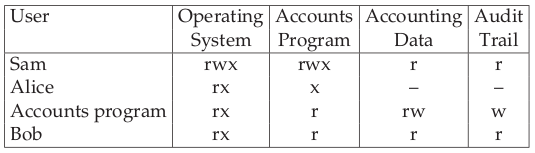
\includegraphics[scale=0.6]{pics/access2.png}
		\end{figure}

		Another way of expressing a policy of this type would be with access triples
		of (user, program, file). In the general case, our concern isn’t with a program
		so much as a protection domain which is a set of processes or threads which
		share access to the same resources.
		Access control matrices (whether in two or three dimensions) can be used to
		implement protection mechanisms as well as just model them. But they do not
		scale well. For instance, a bank with 50,000 staff and 300 applications would
		have an access control matrix of 15,000,000 entries. 

		The two main ways of doing this are to compress the users and to compress the rights. 
		As for the first of these, the 	simplest is to use groups or roles to manage the 
		privileges of {\bf large sets of users} simultaneously, while in the second we may 
		store the access control matrix
		either by {\bf columns (access control lists)} or {\bf rows (capabilities, sometimes known
		as ‘tickets’)}.

		\subsection{Groups and Roles}
			When we look at large organisations, we usually find that most staff fit into
			one or other of a small number of categories. A bank might have 40 or 50:
			teller, chief teller, branch accountant, branch manager, and so on. Only a few
			dozen people (security manager, chief foreign exchange dealer, . . .) will need
			to have their access rights defined individually.
			So we want a small number of pre-defined groups, or functional roles,
			to which staff can be assigned. 

			{\bf Group and roles:} some people use the words group and role
			interchangeably, and with many systems they are; but the more careful
			definition is that a group is a list of principals, while a role is a fixed set of
			access permissions that one or more principals may assume for a period of time
			using some defined procedure. 


		\subsection{Access Control Lists}

			Another way of simplifying the management of access rights is to store the
			access control matrix a column at a time, along with the resource to which
			the column refers. This is called an access control list or ACL (pronounced
			‘ackle’).

			\begin{figure}[H]
				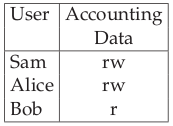
\includegraphics[scale=0.6]{pics/accessControlLists.png}
			\end{figure}

			ACLs have a number of advantages and disadvantages as a means of
			managing security state:

			\begin{itemize}
				\item ACLs are a natural choice in environments where users manage their
				own file security, and became widespread in the Unix systems. They are 
				the basic access control mechanism in Unix-based systems such as GNU/Linux and Apple’s OS/X; the access controls in Windows are also based on ACLs, 
				but have become more complex over time. 
				\item Where access control policy is set centrally, ACLs
				are suited to environments where protection is data-oriented; they are less
				suited where the user population is large and constantly changing, or where
				users want to be able to delegate their authority to run a particular program
				to another user for some set period of time. 
				\item ACLs are simple to implement, but are not efficient as a means of doing security checking at runtime.
				\item Finally, distributing the access rules into ACLs means that it can be tedious
				to find all the files to which a user has access.
			\end{itemize}

		\subsection{Unix OS Security}

			In Unix (including its popular variant Linux), files are not allowed to have
			arbitrary access control lists, but simply rwx attributes for the resource owner,
			the group, and the world. These attributes allow the file to be read, written
			and executed. The access control list as normally displayed has a flag to show
			whether the file is a directory, then flags r, w and x for world, group and owner
			respectively; it then has the owner’s name and the group name. A directory
			with all flags set would have the ACL: \\

				{\bf \color{blue} drwxrwxrwx Alice Accounts} \\


			In the example below: records that the file is not a directory; the file owner can 
			read and write it; group members can read it but not write it; non-group members have 
			no access at all; the file owner is Alice; and the group is Accounts.In our previous example, the ACL of the figure would be: \\

				{\bf \color{blue} -rw-r----- Alice Accounts} \\
				\begin{figure}[H]
					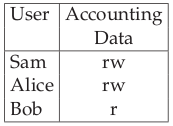
\includegraphics[scale=0.6]{pics/accessControlLists}
				\end{figure}

			In Unix, the program that gets control when the machine is booted (the
			operating system kernel) runs as the supervisor, and has unrestricted access
			to the whole machine. All other programs run as users and have their access
			mediated by the supervisor. 

			This means that (with most flavours of Unix) the system administrator can
			do anything, so we have difficulty implementing an audit trail as a file that
			he cannot modify. This not only means that, in our example, Sam could tinker
			with the accounts, and have difficulty defending himself if he were falsely
			accused of tinkering, but that a hacker who managed to become the system
			administrator could remove all evidence of his intrusion.
			Second, ACLs only contain the names of users, not of programs; so there
			is no straightforward way to implement access triples of (user, program, file).
			Third, ACLs are not very good at expressing mutable state.

		\subsection{Apple's OS/X}

			Apple’s OS/X operating system is based on the FreeBSD version of Unix run-
			ning on top of the Mach kernel. The BSD layer provides memory protection;
			applications cannot access system memory (or each others’) unless running
			with advanced permissions. At the file system level, OS/X is almost a standard Unix.


		\subsection{Windows - Basic Architecture}

			The most widespread PC operating system is Windows, whose protection
			has been largely based on access control lists. 
			
			First, rather than just read, write and execute there are separate attributes for
			take ownership, change permissions and delete, which means that more flexible
			delegation can be supported. These attributes apply to groups as well as users,
			and group permissions allow you to achieve much the same effect as suid
			programs in Unix. Attributes are not simply on or off, as in Unix, but have
			multiple values: you can set AccessDenied, AccessAllowed or SystemAudit. 

			Second, users and resources can be partitioned into domains with distinct
			administrators, and trust can be inherited between domains in one direction
			or both. 

		\clearpage
		\subsection{Capabilities}
			The next way to manage the access control matrix is to store it by rows. These
			are called capabilities. Bob’s capabilities would be:

			\begin{figure}[H]
				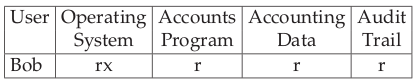
\includegraphics[scale=0.6]{pics/capabilities.png}
			\end{figure}

		The strengths and weaknesses of capabilities are more or less the opposite
		of ACLs. Runtime security checking is more efficient, and we can delegate a
		right without much difficulty. On the other hand, changing a file’s status can 
		suddenly become more tricky as it can be difficult to find out which users 
		have access. This can be tiresome when we have to investigate an incident 
		or prepare evidence of a crime.

	\section{Middleware}
		Doing access control at the level of files and programs was all very well in the
		early days of computing, when these were the resources that mattered. Since
		about the 1980s, growing scale and complexity has meant led to access control
		being done at other levels instead of (sometimes as well as) at the operating
		system level. For example, a bank’s branch bookkeeping system will typically
		run on top of a database product, and the database looks to the operating
		system as one large file. This means that the access control has to be done in
		the database; all the operating system supplies it may be an authenticated ID
		for each user who logs on.

		\subsection{Database Access Control}
			The databases now contain much of the data of greatest relevance to our lives 
			— such as bank accounts, vehicle regis-trations and employment records — 
			and front-end failures sometimes expose the database itself to random online users.
			Database products, such as Oracle, DB2 and MySQL, have their own access
			control mechanisms. As the database looks to the operating system as a single
			large file, the most the operating system can do is to identify users and to
			separate the database from other applications running on the same machine.

		\subsection{General Middleware Issues}
			There are a number of aspects common to middleware security and application-
			level controls. The first is {\bf granularity:} as the operating system works 
			with files, these are usually the smallest objects with which its access control mechanisms can deal. The second is {\bf state}. An access rule such as ‘a nurse can 
			see the records of any patient on her ward’ or ‘a transaction over \$100,000 
			must be authorised by a manager and an accountant’ both involve managing state.
			The third is {\bf level:} we may end up with separate access control systems at 
			the machine, network and application levels, and as these typically come from 
			different vendors it may be difficult to keep them consistent.


			Ease of administration is often a critical bottleneck. In companies the 
			administration of the operating system and the database system
			have been done by different departments, which do not talk to each other;
			and often user pressure drives IT departments to put in crude hacks which
			make the various access control systems seem to work as one, but which open
			up serious holes. An example is ‘single sign-on’. 

			Despite the best efforts of computer managers, most large companies accumulate 
			systems of many different architectures, so users get more and more logons to 
			different systems and the cost of administering them escalates. 
			Many organisations want to give
			each employee a single logon to all the machines on the network. 
			Commercial solutions may involve a single security server through which all 
			logons must pass, and the use of a smartcard to do multiple authentication 
			protocols for different systems. Such solutions are hard to engineer properly, 
			and the security of the best system can very easily be reduced to that of the worst.

		\subsection{ORBs and Policy Languages}
			Problems with middleware led researchers to look for ways in which access control 
			for a number of applications might be handled by standard middleware. Research
			in the 1990s focussed on object request brokers (ORBs). An ORB is a software
			component that mediates communications between objects.
			An ORB typically provides a means of controlling calls that are made across 
			protection domains. The Common Object Request Broker Architecture (CORBA) is an 
			attempt at an industry standard for object-oriented system.

			Languages to express security policy, with projects such as XACML (Sun), XrML 
			(ISO) and SecPAL (Microsoft).

		\subsection{Sandboxing and Proof-Carrying Code}
			The late 1990s saw the emergence of yet another way of implementing access
			control: the software {\bf sandbox}. 
			The model is that a user wants to run some code that she has downloaded 
			from the web as an applet, but is concerned that
			the applet might do something nasty, such as taking a list of all her files and
			mailing it off to a software marketing company.
			The designers of Java tackled this problem by providing a ‘sandbox’ for such
			code — a restricted environment in which it has no access to the local hard
			disk, and is only allowed to communicate with the host it came from.

			An alternative is {\bf proof-carrying code}. Here, code to be executed must carry
			with it a proof that it doesn’t do anything that contravenes the local security
			policy. This way, rather than using an interpreter with the resulting speed
			penalty, one merely has to trust a short program that checks the proofs
			supplied by downloaded programs before allowing them to be executed.

		\subsection{Trusted Computing}
			The ‘Trusted Computing’ initiative was launched by Microsoft, Intel, IBM, HP
			and Compaq to provide a more secure PC. Their stated aim was to provide
			software and hardware add-ons to the PC architecture that would enable
			people to be sure that a given program was running on a machine with a
			given specification; that is, that software had not been patched (whether by
			the user or by other software) and was running on a identifiable type and
			configuration of PC rather than on an emulator. The initial motivation was
			to support digital rights management.


	\clearpage
	\section{Hardware Protection}
		--Write something?--





